\documentclass[
tikz,
border=5pt,
convert={density=600,
	outext=.png
}
]{standalone}


\usepackage[utf8]{inputenc}
%\usepackage{/home/ccaprani/projects/Tikz-StructuralAnalysis/stanli.sty}
\usepackage{stanli}
\usepackage{tikz}
\usetikzlibrary{arrows.meta,arrows,positioning,calc,backgrounds}

\begin{document}
	
	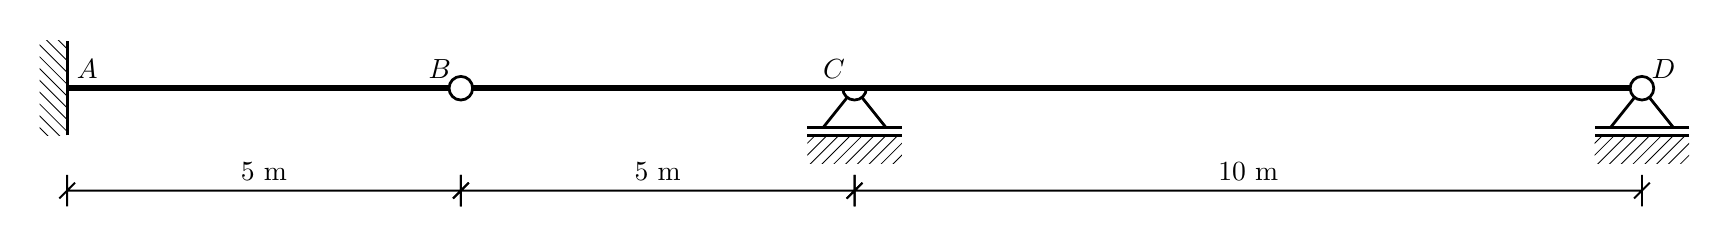
\begin{tikzpicture}[background rectangle/.style={fill=white!45}, show background rectangle]
		
		% Draw beam, supports, notation
		% Stations
		\point{a}{0}{0};
		\point{b}{5.0}{0};
		\point{c}{10.0}{0};
		\point{d}{20.0}{0};
		
		% Draw the beam between the stations
		\foreach \startn/\endn in {a/b,b/c,c/d}
			\beam{4}{\startn}{\endn};
		
		% Supports
		\support{3}{a}[-90];
		\support{2}{c};
		\support{2}{d};		
		
		% hinges
		\foreach \startpt in {b,d}
			\hinge{1}{\startpt};
		\hinge{2}{c}[b][d];
		
		% Dimensions
		\dimensioning{1}{a}{b}{-1.3}[$5$~m];
		\dimensioning{1}{b}{c}{-1.3}[$5$~m];
		\dimensioning{1}{c}{d}{-1.3}[$10$~m];
		
		% Letters - no ticks = 1; ticks = 2
		\notation {1}{a}{$A$}[above right];
		\notation {1}{b}{$B$}[above left];
		\notation {1}{c}{$C$}[above left];
		\notation {1}{d}{$D$}[above right];
		
	\end{tikzpicture}
	
\end{document}